%!TEX root = dippa.tex
%%% This file contains the results section of my master's thesis.
%%% Author: Viljami Aittomäki

\section{Results}

The results of performed analyses are presented as follows. First,
summaries on quality control and correlation analyses between the different
data types are presented, followed by results from regression model simulations.
Finally, the performance of projection prediction and lasso regression
is compared from a target prediction perspective.




\subsection*{Quality control}

Quality-control plots are presented in Appendix \ref{app:qc-plots}. 
The preprocessed protein and mRNA expression data appeared reasonably uniform
and approximately Gaussian, though several variables had long tails
and a few had significant outliers (most notably proteins CDK1, ERRFI1, PIK3CA).
This was most apparent in the scaled data. miRNA microarrays had strongly bimodal
distributions, there was large variation in miRNA variable median expression,
and many miRNA variables were highly skewed towards very small values.
There appeared to be quantification artifacts in the miRNA variables.

This is indicative of generally low abundances of some miRNA molecules
and, although partly due to different preprocessing compared to the mRNA and
protein arrays, it raises suspicion of significant noise in the miRNA data.

The first two principal components for each data type are plotted in Figure
\ref{fig:qc-pca}. No significant batch effect was visible. The hierarchical
clustering of samples (not shown) had a similar result.




\subsection*{Correlation analysis}

Pearson correlations between variables from the different data types are shown in Figure
\ref{fig:correlations}. Protein-mRNA correlation was clearly higher for gene-matched pairs
(that is protein and mRNA expression corresponding to the same gene) than unmatched pairs,
and correlations for unmatched pairs were concentrated around zero, both expected
results. Notably, even the gene-matched correlations were quite low, with a
mean $\bar{\rho} \approx 0.37$. Using the squared correlation coefficient $\rho^2$ as a
measure of explained variance (although this has been criticized), the amount
of protein variance explained by the matched mRNA ranged from 0\% to 82\% with a mean of
21\%.

\begin{figure}[!h]
  \centering
  \begin{subfigure}{.45\textwidth}
    \subcaption{ \label{fig:protein-gene-cor}}
    \centering
    \includegraphics[width=1\linewidth]{figures/correlationPlots/protein-gene-correlation.pdf}
  \end{subfigure}
  \begin{subfigure}{.45\textwidth}
    \subcaption{ \label{fig:protein-mirna-cor}}
    \centering
    \includegraphics[width=1\linewidth]{figures/correlationPlots/protein-mirna-correlation.pdf}
  \end{subfigure}
  \begin{subfigure}{.45\textwidth}
    \subcaption{ \label{fig:gene-mirna-cor}}
    %\centering
    \includegraphics[width=1\linewidth]{figures/correlationPlots/gene-mirna-correlation.pdf}
  \end{subfigure}

  \caption{Distributions of Pearson correlations between variables of different expression data types.
  The distributions are trimmed at the smallest and largest values.
  (a) Correlation between protein and mRNA pairs, where "matched" refers to correlating
  protein and mRNA from the same gene.
  (b) Correlation between protein and miRNA pairs, where "validated" refers to the gene
  being a validated target of the miRNA (according to TarBase),
  and "random" to a randomly picked group of protein-miRNA pairs.
  (c) Correlation between mRNA and miRNA pairs,
  where grouping is the same as in (b).}
  \label{fig:correlations}
\end{figure}

Correlations between miRNAs and their validated target genes (fetched from
TarBase) were mostly low with no preference towards negative (or positive)
values. There was virtually no difference in correlations between validated
targets and randomly picked gene-miRNA pairs, contrary to what might be
expected.




\subsection*{Model simulations}

Simulations for the cross validation (to determine model size) lasted
between 4 to 6 hours (on a computing-cluster node with 2 12-core Xeon E5 2680
2.50GHz processors), and simulations for the final projected models lasted
between 2 to 45 minutes, depending on the chosen model size. All parameters for all
simulations had low potential scale reduction $\hat{R}^2 < 1.1$, indicating
good convergence of simulation chains \citep{Gelman2013}.

The parameters for the model-size criterion, $\alpha$ and $\gamma$, had a
significant effect on the resulting model sizes (a plot of model-size
distributions is shown in Appendix \ref{app:model-sizes}).
Values $\alpha = 0.50$ and $\gamma = 0.2$ were chosen to keep models
relatively sparse. This choice was, however, largely subjective.

Out of the
105 genes in the data, a projected model (where at least one miRNA variable
was included, and the model-size criterion was met in under 200 variables) was
found for 74 genes. Figure \ref{fig:forward-search} shows the predictive performance during the
forward search in cross validation for one of the best performing models (\emph{CDH3})
and one of the worst (\emph{PIK3CA}).
A table of properties for the projected models is
available in Appendix \ref{app:model-table}.

\begin{figure}[!h]
  \centering
  \begin{subfigure}{.45\textwidth}
    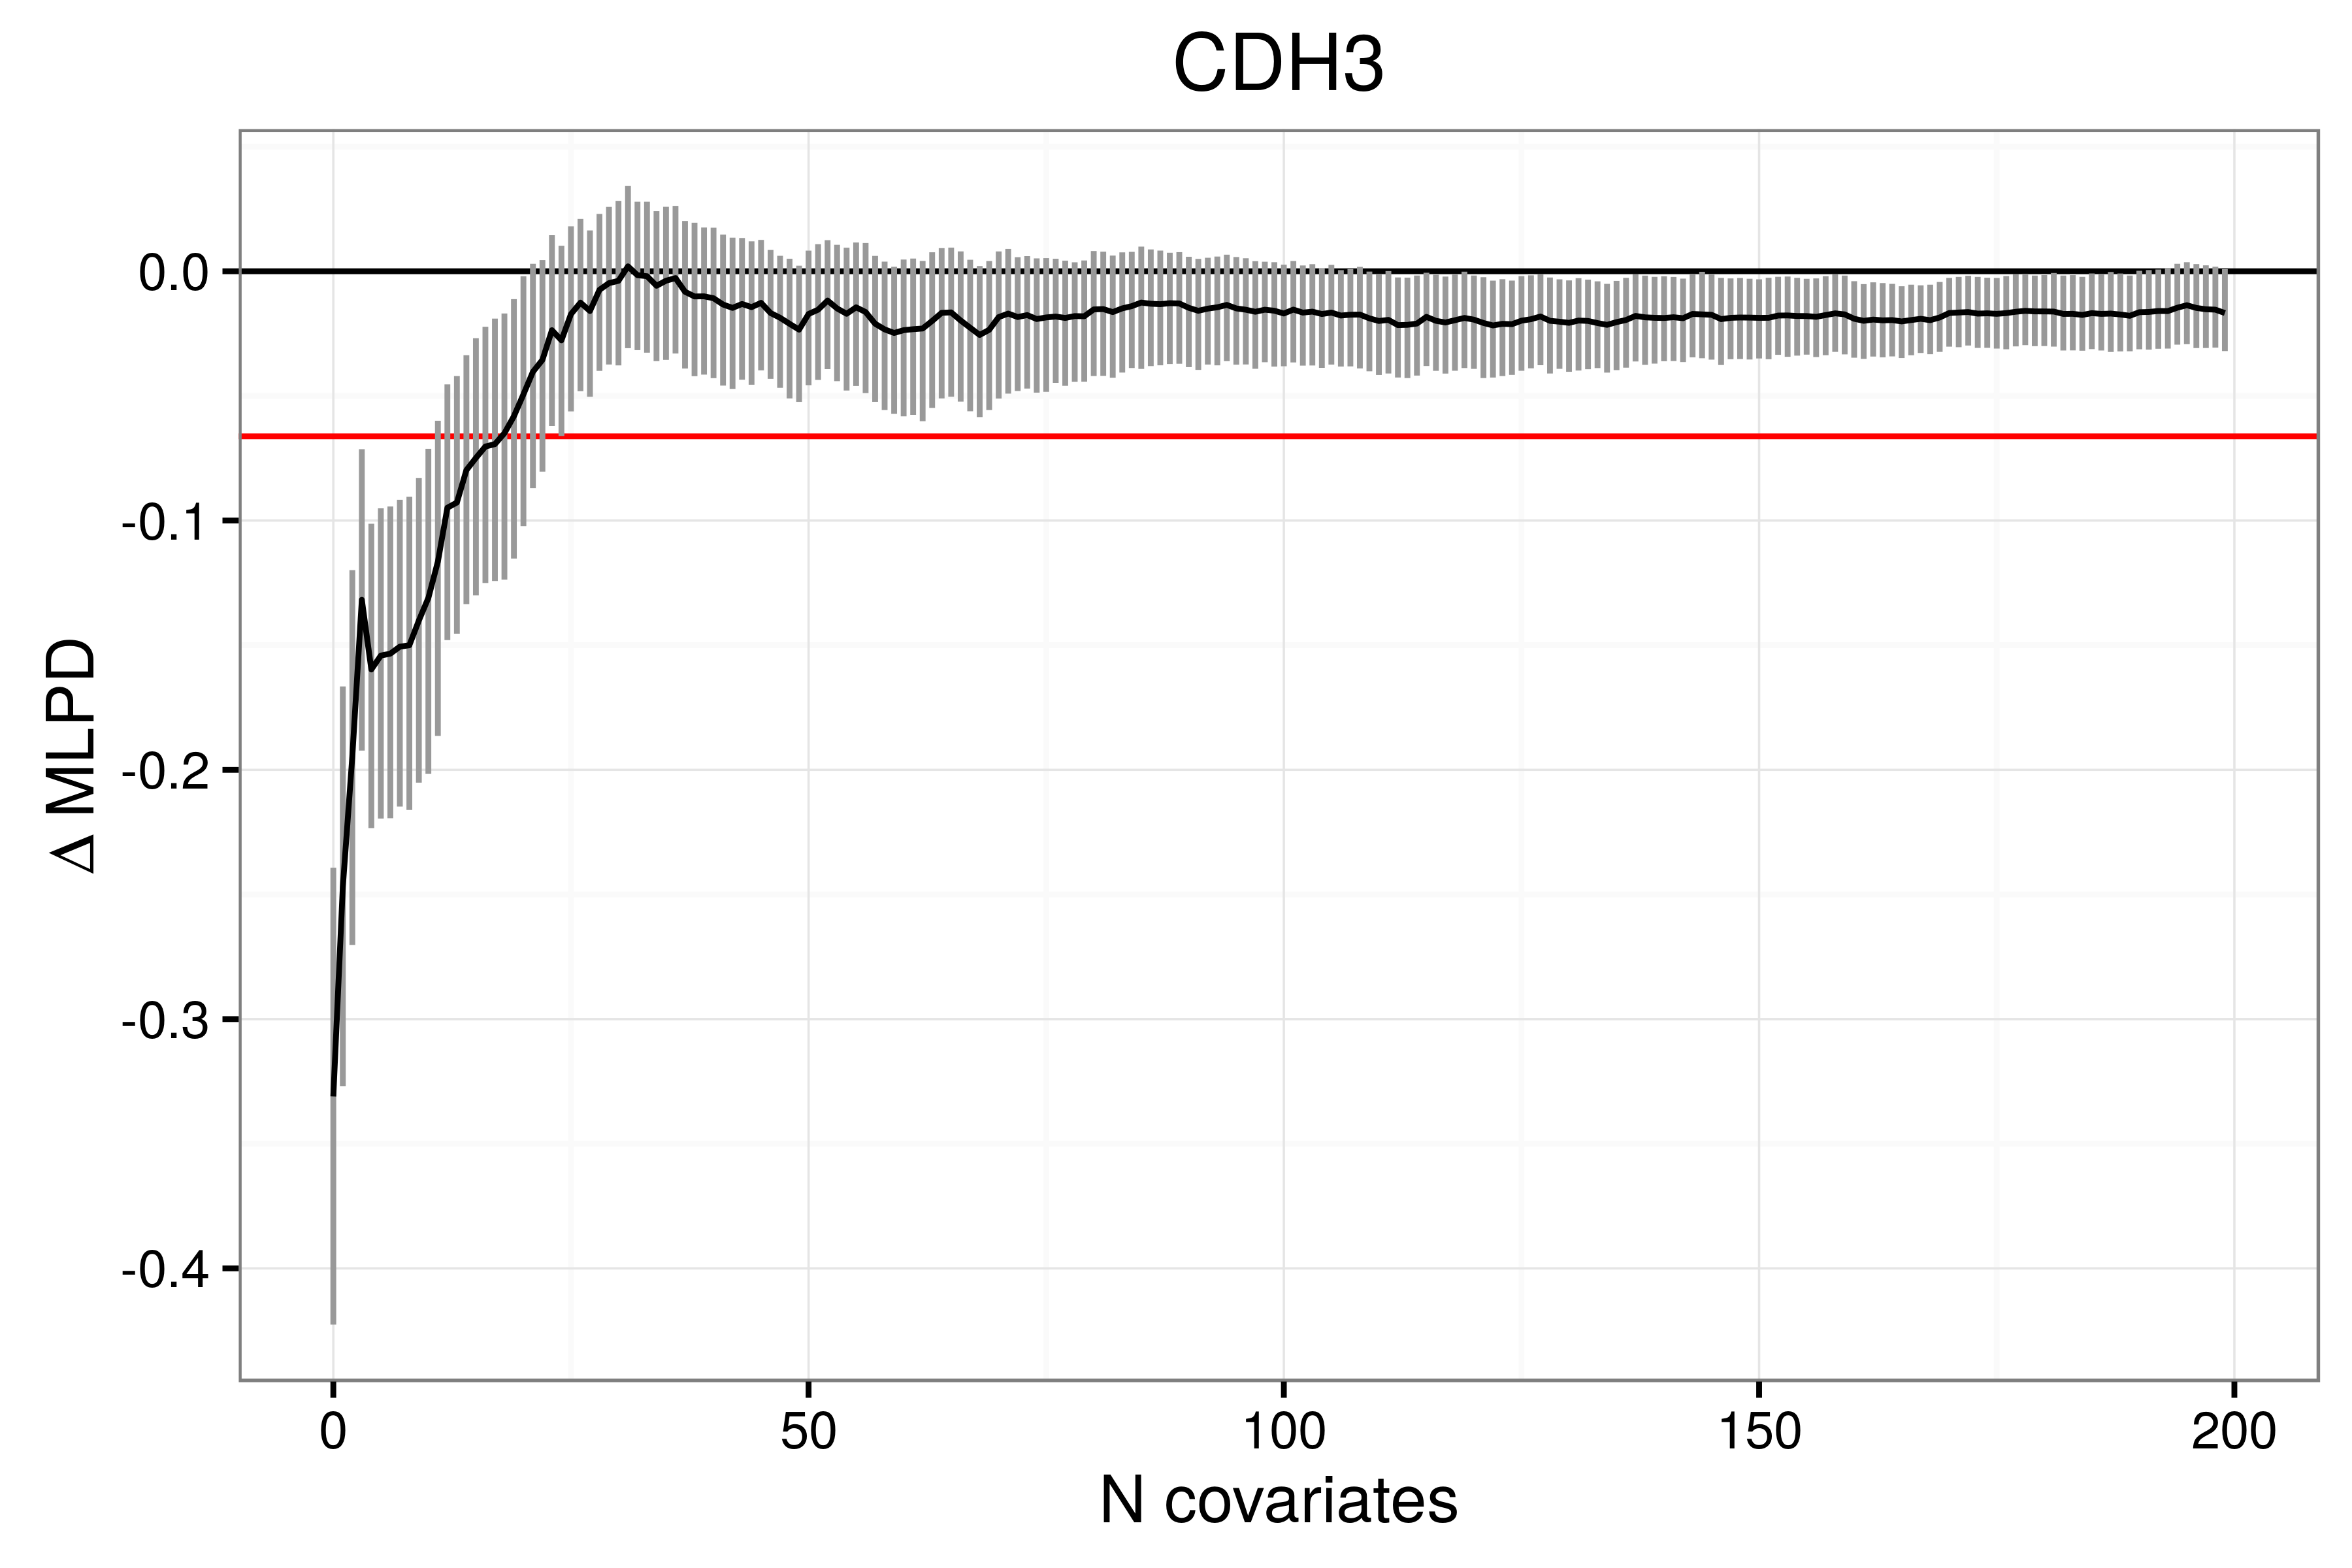
\includegraphics[width=1\linewidth]{figures/CDH3_CV_path.png}
  \end{subfigure}
  \begin{subfigure}{.45\textwidth}
    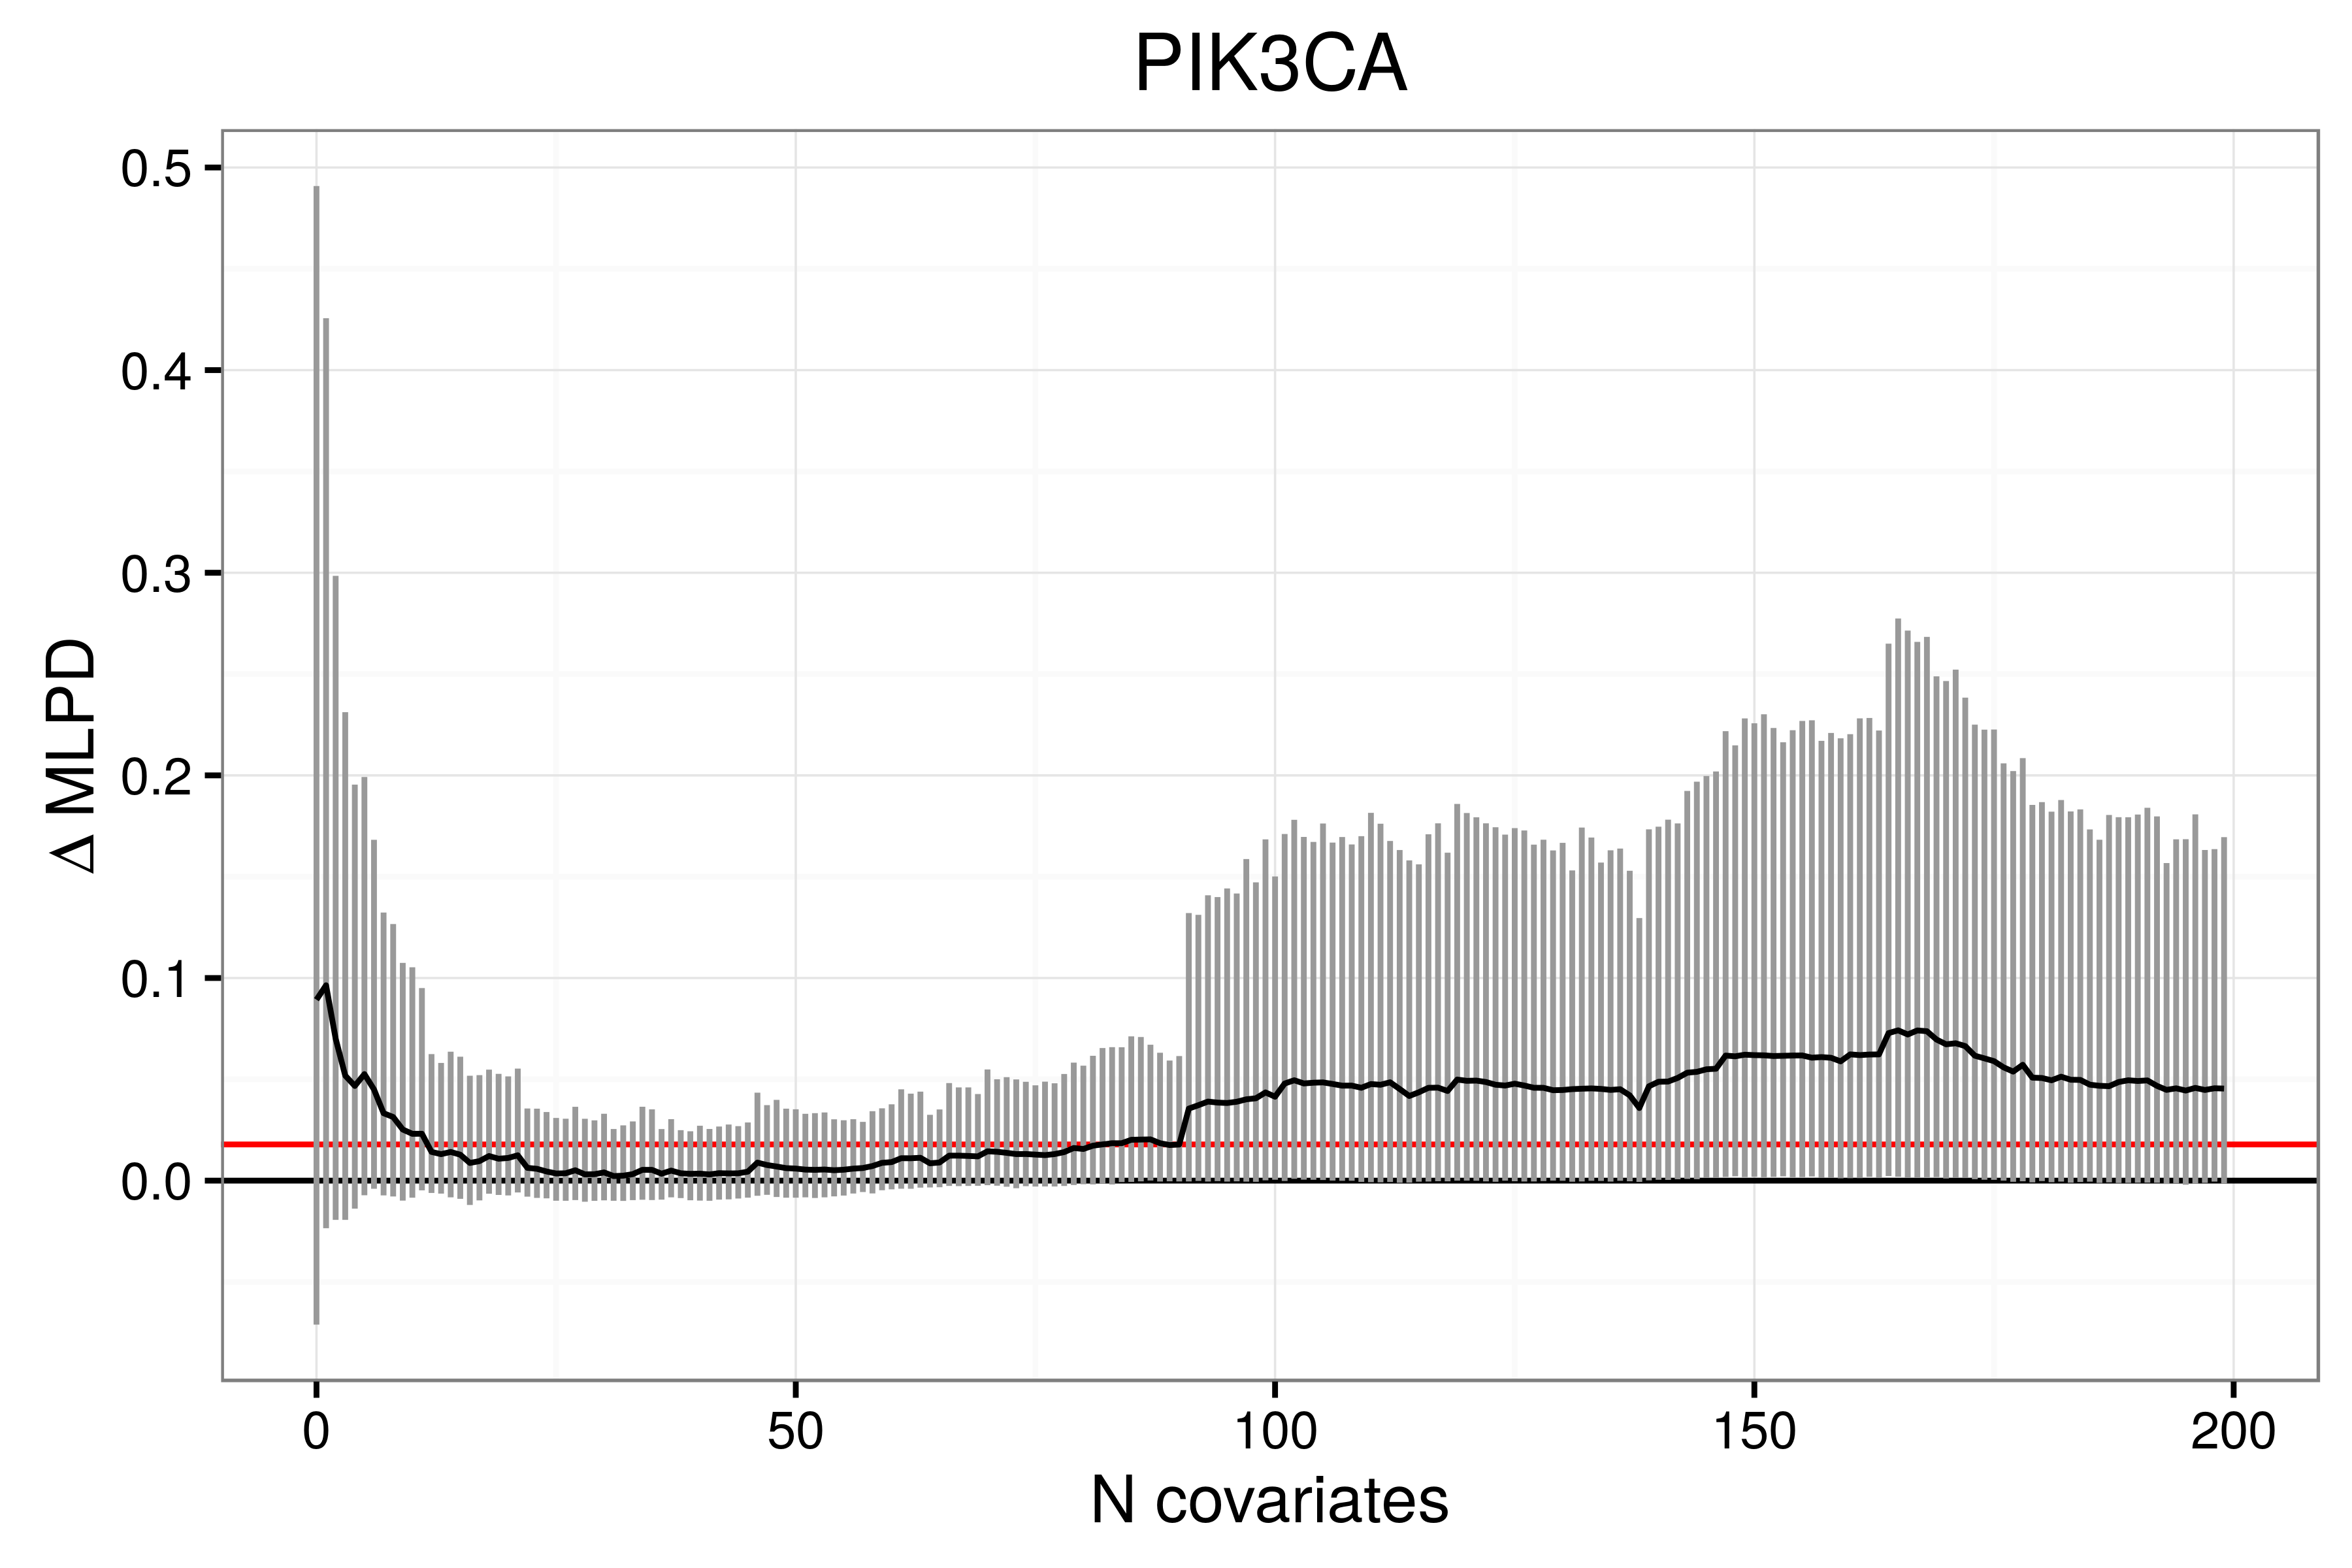
\includegraphics[width=1\linewidth]{figures/PIK3CA_CV_path.png}
  \end{subfigure}

  \caption{Predictive performance ($\Delta\textup{MLPD}$) of projected submodel $M_\perp$ during
  each step of the forward search in the model-size-selection phase. Two of the 105 models are shown.
  The black line shows the median (corresponding to $\alpha = 0.50$) and
  gray lines the 95\% interval of $\Delta\textup{MLPD}$ computed with Bayesian bootstrap.
  The red line depicts the model-size selection threshold $U$ (with $\gamma=0.2$).
  The final \emph{CDH3} model was one of the best performing ones,
  no model was found for \emph{PIK3CA}, as the intercept-only model
  already performed better than the full model.}
  \label{fig:forward-search}
\end{figure}

Figure \ref{fig:n-miRNAs-vs-R2} shows the number of miRNA variables included in
each projected model plotted against the number of significant miRNA
variables, the $R^2$ of the projected model, and the difference in $\bar{R}^2$
between the projected model and the gene-only model. Each point in each plot
corresponds to one gene. A trend emerged, where including more
miRNA variables tended to achieve better model performance up to a turning point --
around 28 miRNA variables -- after which larger models seemed to perform
increasingly poorly. Similar plots were created with more strict model-size
thresholds (larger $\alpha$ and smaller $\gamma$); the models were larger on
average, but an equal trend and turning point were observed (data not shown).

\begin{figure}[!h]
  \centering
  \includegraphics[height=11cm]{figures/n_miRNAs_vs_R2.pdf}
  \caption{Size of final model compared to model goodness-of-fit. The x-axis is
  the total number of chosen miRNA variables in each final projected model (N miRNAs).
  The three y-axes show the number of significant miRNA variables (N significant miRNAs),
  $R^2$ of the projected model, and the
  difference in $\bar{R}^2$ between the projected and gene-only models
  ($\Delta\bar{R}^2$). Each point represents one model fitted for one gene. A
  small jitter has been added to the points on the x-axis to help visualize all of them.
  Curves were fitted with locally weighted scatter plot smoothing (LOESS) and
  shaded areas represent 95\% confidence interval. A trend can be seen, where
  models larger than approximately 28 included miRNAs perform increasingly poorly.}
  \label{fig:n-miRNAs-vs-R2}
\end{figure}

Lasso regression produced models with at least one miRNA for 74 genes, out of
which only 57 were common to the ones found by projection prediction (PPVS).
For 18 of the lasso models, the mRNA expression variable was not included.
Figure \ref{fig:model-size} shows a comparison of model size distribution
and $\Delta\bar{R}^2$ between PPVS and lasso.

\begin{figure}[!h]
  \centering
  \begin{subfigure}{.45\textwidth}
    \includegraphics[width=1\linewidth]{figures/R2comparison/n_miRNA_comparison.pdf}
  \end{subfigure}
  \begin{subfigure}{.45\textwidth}
    \includegraphics[width=1\linewidth]{figures/R2comparison/R2_comparison.pdf}
  \end{subfigure}

  \caption{Comparison of model sizes (shown left) and $\Delta\bar{R}^2$ (shown right) for
      projection prediction (PPVS) and lasso regression.}
  \label{fig:model-size}
\end{figure}




\subsubsection*{Target prediction performance}

Considering each selected miRNA variable as a putative miRNA-mRNA target
interaction, PPVS generated a total 945 target predictions, out of which
253 were significant (on a 95\% posterior interval). Table \ref{table:final-models}
lists the significant predictions.
Lasso regression generated all together 650 target predictions. Figure
\ref{fig:venn} shows the overlap of predictions by PPVS and lasso, and also
that of significant predictions from PPVS and the same number of top
predictions from lasso, where lasso predictions were ranked by the absolute value of
the regression coefficient.\footnote{Lasso regression does not provide any
rank measures or tests of significance.}

\begin{figure}[!h]
  \centering
  \begin{subfigure}{.45\textwidth}
    \centering
    \includegraphics[width=1\linewidth]{figures/compareModels/Venn-PPVS-lasso.pdf}
  \end{subfigure}
  \begin{subfigure}{.45\textwidth}
    \centering
    \includegraphics[width=1\linewidth]{figures/compareModels/Venn-PPVS_sig-lasso_top.pdf}
  \end{subfigure}

  \caption{Venn diagrams showing the overlap of target predictions from PPVS
  and lasso (shown left). Shown right is the overlap of significant predictions
  from PPVS and the same number of top predictions from lasso (ranked by
  absolute value of regression coefficient).}
  \label{fig:venn}
\end{figure}

Figure \ref{fig:scatter-ppvs-lasso} shows a comparison of the regression
coefficients from PPVS and lasso for targets predicted by both methods. There
were only three predicted targets for which the methods did not agree on the
sign of the coefficient. PPVS produced larger coefficients in general, and
correlation for the coefficients was fairly high ($0.86$).

\begin{figure}[htb]
  \centering
  \includegraphics[width=.6\linewidth]{figures/compareModels/Scatter-PPVS-lasso.pdf}
  \caption{Scatter plot of miRNA regression coefficients from projection
  prediction (PPVS) and lasso for the 145 common targets predicted by both methods.
  Note that PPVS coefficients generally have greater magnitude. Triangles
  mark significant coefficients in PPVS. The gray
  line marks unity ($x=y$).}
  \label{fig:scatter-ppvs-lasso}
\end{figure}

PPVS and lasso had similar performance in regards of discovering validated
targets: approximately 12\% of PPVS and 14\% of lasso predictions were present
in the union of TarBase and miRTarBase. These proportions were 13\% and 14\% for
the significant PPVS and top lasso predictions, respectively. Therefore,
limiting predictions to the ones with most confidence did not significantly increase
the proportion of validated targets for either method.

For both methods, approximately half of the coefficients for both all
predicted and validated targets were positive, indicating upregulation by the
miRNA. In contrast, in TarBase, all of the discovered validated interactions
were classified as downregulative. miRTarBase does not provide data on the
nature of the regulation.
